% -*- root: ../../main.tex -*-
%!TEX root = ../../main.tex
% vim:textwidth=80 fo=cqt

\glsreset{rom}

Battery  modellers face  the  classic conundrum  of  conjuring \glspl{pbm}  that
remain  amenable  for control  applications.  The  prior  attempts made  by  the
research  community  to  tackle  this  challenge  is  examined  here.  The  term
`control-oriented model' can  be considered synonymous with  the term \gls{rom}.
This  is  due  to  the  fact  that  the  complexity  of  \glspl{pbm}  inherently
necessitates the  use of  some order  reduction strategy  for their  adoption in
control and  real-time applications. In this  thesis as well as  in the relevant
literature discussed here, these two terms have been used interchangeably.

Research   into  \glspl{rom}   is  motivated   by  the   pressing  need   for  a
real-time   model   with   accuracy   properties   of   full-order   \glspl{pbm}
but   possessing    the   computational    simplicity   of    \glspl{ecm}   (see
\crefrange{subsec:ecms}{subsec:pbms} for  an overview).  A number  of approaches
to  reduce  the  computational  complexity of  \glspl{pbm}  have  been  explored
in  literature.  Jokar~\etal~\cite{Jokar2016}  provide  a  comprehensive  review
of  the  various  categories  of  reduced  order  \glspl{pbm}  for  lithium  ion
batteries.  However,  the  aforesaid  work  does  not  aim  to  classify  models
based  on  time-vs-frequency  domains.  Fan~\etal{}~\cite{Fan2015}  conducted  a
review  of  reduced  order  modelling   methods,  but  only  provide  a  generic
overview of  deriving and implementing models  in these dual domains  without an
expository  analysis of  the  implications of  these  modelling choices.  Unlike
Jokar~\etal~\cite{Jokar2016}, the review by Fan~\etal{} did not aim to provide a
classification  of various  reduced order  models, but  instead emphasises  on a
broad survey of relevant methodologies  and tools towards \emph{obtaining} them.
Hence,  neither  of  these  works  provide  an  insight  into  the  rubrics  and
implications  of  the  choice  of  either  of  these  domains  to  underpin  the
\glspl{rom}. Although  in principle,  the transformation  between them  is often
a  straightforward  mathematical  exercise,  availability of  models  for  final
implementation in the time domain aids immediate uptake by industry for adoption
in  online \glspl{bms}.  The treatment  of \glspl{rom}  from this  aspect is  so
germane to the central hypothesis of this  thesis (a simple time domain model is
the  key to  large scale  deployment of  \glspl{pbm}), that  the author  of this
thesis feels  compelled to  undertake a simpler  classification exercise  of the
existing  modelling art,  within the  context  of their  suitability for  online
implementation.


In this discussion,  various modelling methodologies and  their resultant models
are viewed as  a single continuum. Consequently this thesis  discusses them from
such a  unified perspective without  microscopic separation of the  final models
from their progenitor mathematical methods. Furthermore, there is also a need to
highlight the salient works among the more recent advances and extensions to the
then  prevailing models  to obtain  an updated  view of  the modelling  art that
have  gained  traction  since the  publication  of  Jokar~\etal~\cite{Jokar2016}
and  Fan~\etal~\cite{Fan2015}. Hence,  the specialised  review of  reduced order
modelling  literature  covered  in  this  section  intends  to  supplement,  not
supplant,  the breadth  of  research  covered between  the  aforesaid works.  In
particular, care has been taken to minimise repetition of background art already
analysed in these aforementioned review articles, thereby striving to report the
subset of prior research that is  pertinent to illustrate the new classification
scheme introduced  here. The author  does not aim  to adhere to  a chronological
presentation of such  background works. Instead, salient  \gls{rom} families are
introduced  in  the  context  of  discussion  of  their  significance  within  a
particular mathematical modelling technique.


In the views of this thesis author, physics-based control-oriented models can be
classified as belonging to one of the following categories
% \begin{itemize}[topsep=0pt, partopsep=0pt, parsep=0pt, itemsep=0pt]
\begin{itemize}
    \item Frequency domain \glsfmtshortpl{rom}
    \item Quasi-hybrid time/frequency domain \glsfmtshortpl{rom}
    \item Hybrid \glsfmtshortpl{rom} based on equivalent circuits
    \item Time-domain \glsfmtshortpl{rom}
\end{itemize}
A common characteristic of all control-oriented models is that their ultimate
goal is to lower the computational burden of the pertinent physical quantities
during operation of the cell.  However upon a closer study, a few contrasting
aspects that set them apart become apparent. Understanding the behavioural
differences that stem from their lineage is the motive behind distinguishing
between those models that are derived directly in the time  domain versus  those
that  are derived first  in the  frequency domain, but  later  converted  to
time  domain.

The classical \mbox{modus operandi} in frequency domain modelling is to
transform the underlying physical equations into the Laplace space (the complex
S~plane) followed by a Padé approximation to reduce the number of coefficients
in the resulting transfer functions. This category of models is briefly
evaluated in \cref{subsec:freqdomainroms}. At the other end of the spectrum are
the time-domain \glspl{rom} which typically adopt the strategy of either
\begin{enumerate*}[label=\itshape\alph*\upshape)]
    \item simplifying the computational mesh used,
    \item capturing only the salient dynamics of the cell which leads to a smaller parameter set,
        and/or
    \item a combination of the two.
\end{enumerate*}
The state of the art in these models is studied in \cref{subsec:timedomainroms}.
An overlapping continuum of mathematical techniques is encountered in the
literature discussing the wide assortment of \glspl{rom} spanning the
intervening space between these extrema. The classification presented here
reflects their broad approach to model reduction. For instance, equivalent
circuits have only a few parameters and are an attractive option from an
implementation perspective. In recent years, there has been an up~trend in
published efforts employing mathematical methods to generate physics-based
equivalent circuits, the salient among which are discussed in
\cref{subsec:hybridroms}. Finally, there exist Quasi-hybrid \glspl{rom} which do
not necessarily seek to formulate equivalent circuits, but rather strive to
arrive at  time domain reduced order state-space realisations by proceeding
through a series of mathematical transformations starting from the frequency
domain. In these models, order reduction is typically achieved through a
reduction in the number of \emph{states} and not directly through a reduction in
the number of parameters. These methods typically  employ both time-domain and
frequency-domain aspects of control theory, such as Markov parameters and the
Ho-Kalman algorithm. An evaluation of the salient quasi-hybrid \glspl{rom} from
literature is presented in \cref{subsec:quasiroms}.


In  principle, any  modelling  method  that yields  a  time domain  mathematical
description  of physical  phenomena that  is lower  in computational  complexity
by  some  arbitrary   magnitude  than  the  original  \gls{dfn}   model  can  be
considered  as  a  candidate  for  further  investigation.  In  the  absence  of
a  canonical  or  quantitative  definition  of  what  constitutes  a  \gls{rom},
the  number  of  candidate  family  of  models  to  consider  is  overwhelmingly
large.  In  practice,  the  constraint  imposed   by  the  scope  of  this  work
\ie~suitability  for real-time  implementation, limits  the choice  of candidate
modelling  families.  For  instance,   models  relying  primarily  on  classical
finite  difference~\cite{Smith2006}, Galerkin's  approximation~\cite{Dao2012} or
Galerkin's  projection~\cite{Fan2016,Fan2018}  methods  for  transformation  and
order  reduction of  one or  more  field variables  of the  \gls{dfn} model  are
excluded from  further study. This  is done in  view of the  impracticability of
implementing  such  models in  a  resource-constrained  environment such  as  an
embedded \gls{bms} controller.

\subsection{Frequency   domain   \glsfmtshortpl{rom}}\label{subsec:freqdomainroms}

Owing  to the  low entry-barrier  for adoption  in a  real-time controller  that
typically logs data samples at  specific time intervals, this thesis prioritises
those models  that are cast in  a mathematical form directly  suitable for final
implementation in  the time domain. This  choice implies the exclusion  of those
models that  are derived and implemented  entirely in the frequency  domain. For
the sake of readers interested in  frequency domain methods, the discussion here
briefly introduces  salient literature  employing the Padé  approximation method
that serves as a backbone of a wide variety of frequency domain models.


The     transfer     function     oriented     Padé     approximation     method
for    low    order    physics-based     battery    modelling    pioneered    by
Forman~\etal{}~\cite{Forman2011a}    has   gained    widespread   adoption    in
the    areas     of    cell     design~\cite{Marcicki2013},    charge-trajectory
optimisation~\cite{Bashash2010},    controller    design~\cite{Perez2015}    and
state    estimation~\cite{Marcicki2013,Moura2012}.     Although    Prasad    and
Rahn~\cite{Prasad2013} present  an online identification  of a subset  of ageing
parameters  using  a Padé  model  and  the  \gls{rls}  algorithm,
specific implementation details  such as the transformation of  the Padé reduced
impedance to discrete-time  difference equations were not  provided. Padé models
are typically limited to offline applications owing to the aggressive trade-offs
required in  its approximation order  so as  to maintain high  accuracies. Those
models truncated  to very low  Padé order exhibit  poor fidelity and  perform no
better  than  classical  \glspl{ecm},  although recent  research  attempts  have
focused to mitigate this drawback~\cite{Yuan2017a,Yuan2017}.


\subsection{Quasi-hybrid time/frequency domain \glsfmtshortpl{rom}}\label{subsec:quasiroms}

Smith~\etal{}~\cite{Smith2007} pioneered a semi-hybrid approach to reduced order
modelling and  obtained closed  form expressions  for all  electrochemical field
variables  in  the frequency  domain  except  for those  describing  electrolyte
concentration and  potential (which were  solved separately using  the classical
finite  difference  discretisation  method).  To the  author's  knowledge,  this
is  the  earliest published  instance  wherein  all  the  dynamics of  the  full
order  model  were  completely  retained  in  the  frequency  domain.  This  was
facilitated through  the use  of transcendental  transfer functions  that helped
to  avoid  the  accuracy  degradation brought  about  by  truncation  techniques
such  as  Padé  approximation.  In  the first  stage  of  the  model  derivation
detailed in  the said  article, a  composite impedance  model for  the frequency
range  of interest  from  \SIrange{0}{10}{\hertz} was  obtained.  This was  then
converted to a \engordnumber{12} order state  space model using the technique of
residue  grouping  and  truncation,  thereby demonstrating  the  first  instance
of  the   so-called  hybrid  modelling   workflow.  The  \gls{rom}   derived  in
Smith~\etal{}~\cite{Smith2007}  was capable  of predicting  the cell's  terminal
voltage within \SI{1}{\percent} of the full-order \gls{dfn} model.

The  modelling  effort by  Smith~\etal{}~\cite{Smith2007}  also  has the  unique
distinction of being  the first of its  kind to render a  \gls{pbm} suitable for
implementation in the classical \gls{lti} state-space formulation
\begin{equation}\label{eq:LTIstatespace}
    \begin{aligned}
        \dot{\mathbf{x}} &= A\,\mathbf{x} + B\,\mathbf{u} \\
        \mathbf{y} &= C \, \mathbf{x} + D\, \mathbf{u},
    \end{aligned}
\end{equation}
\begin{flalign}
    \text{where   }    \mathbf{x}   \in   \mathbb{R}^{n\times   1},\:    A   \in
    \mathbb{R}^{n\times   n},\:   B  \in   \mathbb{R}^{n\times   m},\:\mathbf{y}
    \in  \mathbb{R}^{p\times  1},\:  C   \in  \mathbb{R}^{p\times  n},\:  D  \in
    \mathbb{R}^{p\times m}\: \text{and }  \mathbf{u} \in \mathbb{R}^{m \times
    1}
    && \notag
\end{flalign}
that is amenable  for controller design and for  further system-level simulation
studies  \eg~as a  component  in  the energy  storage  subsystem  of a  (hybrid)
electric vehicle drivetrain.
% an  \gls{xeV} drivetrain.

The requirement  of a  relatively large  number of  state variables  (12~in this
case) for  describing the system's  dynamics dilutes the effectiveness  of state
estimation  algorithms.  In  the  classical isothermal  implementation  of  this
\gls{rom}, with  the cell's terminal  voltage being the only  measured quantity,
the  observability of  the model  degrades significantly.  Although Smith~\etal{}
performed  an  observability analysis  of  the  model  in a  noise-free  context,
the  presence of  process noise  (via unmodelled  electrochemical phenomena  and
parameter uncertainties)  coupled with corruption of  measurement values through
sensor  noise  in  a  harsh  electrical  environment  such  as  in  a  vehicle's
drivetrain, makes  this model  unattractive for state  estimation tasks  in such
embedded applications.


Several attempts have been undertaken to  improve and extend the ideas pioneered
in Smith~\etal{}  For instance,  Lee~\etal{}~\cite{Lee2012a}~addressed a
critical missing aspect \viz~the derivation of transcendental transfer functions
for  both  the  electrolyte  concentration and  its  potential.  These  transfer
functions were  obtained by  using a Sturm-Liouville  approach by  retaining the
first  five modes  of an  eigenfunction  expansion procedure  which is  detailed
in~\cite{Lee2012,Lee2012a}. To  the author's best  knowledge, this is  the first
published  work wherein  all electrochemical  field variables  of the  \gls{dfn}
model were  considered for  inclusion in a  deterministic model  order reduction
procedure whilst keeping the derivation entirely in the frequency domain.


Obtaining closed form expressions for  the electrochemical variables achieved in
Smith~\etal{} (for all quantities other than electrolyte transfer functions) and
Lee~\etal{} (all  quantities including electrolyte transfer  functions) also has
an important computational implication.  With these capstone derivations serving
to complete the  model description in the frequency  domain, all electrochemical
variables  of the  \gls{dfn}  model could  now be  solved  independently at  any
desired spatial location, in particular at certain crucial locations such as the
interface of each electrode with  the respective current collector or separator.
This ground~breaking idea sharply contrasted with the then prevalent state of the
art  in  reduced  order  modelling.  For  the  simplification  of  the  original
\gls{pdae} of  equations in \cref{tbl:dfneqns}, most  order reduction approaches
(excluding the \gls{spm} that shall  be discussed later) invariably required the
solution of all electrochemical quantities  at multiple node locations along the
thickness of  the cell, thereby adding  to the computational burden.  This was a
significant deterrent to  the adoption of such \glspl{rom},  particularly if the
intended purpose of  the model is to simply predict  the cell's terminal voltage
or serve as the plant model in \gls{soc} estimation applications.


In the  same publications~\cite{Lee2012a,Lee2012}, Lee~\etal{} also  devised the
\gls{dra},  a  novel  scheme  to  systematically  transform  all  transcendental
transfer functions to  the time domain so as to  obtain an \gls{lti} state-space
model  given  by  \cref{eq:LTIstatespace}.  The  \gls{dra}  method  retains  the
physical character of the original \gls{dfn}  equations until the very last step
wherein the matrices governing the  system's dynamics are generated. This yields
a one-dimensional  discrete-time \gls{rom}  of the cell  that is  entirely based
upon fundamental  physical principles.  The \gls{rom}  thus obtained  could then
be  used to  compute  the  time-evolution of  all  the internal  electrochemical
quantities of the \gls{dfn} model. As an illustrative application of the method,
Lee~\etal~\cite{Lee2012a} performed a simulation study of
\begin{enumerate*}[label=\itshape\alph*\upshape)]
    \item the reaction flux density,
    \item surface concentration of Li,
    \item ionic concentration of \ch{Li^+} in the electrolyte,
    \item potential in electrolyte, and
    \item potential in solid
\end{enumerate*}
in   the  anode   and  cathode   at   the  respective   domain  boundaries   and
demonstrated  their high  accuracies relative  to a  benchmark \gls{dfn}  model.
In  Lee~\etal~\cite{Lee2012,Lee2012a}, the  cell  voltage  was computed  through
linear  combinations of  these  time-domain variables  with suitable  non-linear
corrections. Yet another advantage of this model order reduction process is that
the method does not involve any  form of non-linear optimisation that is typical
of other order reduction schemes that attempt a top-down approach of simplifying
the \gls{pbm} equations. In  particular, the \gls{dra} scheme provides
a deterministic method for selection of the order of the simplified model, which
is a pioneering  contribution in the field of reduced  order modelling of Li-ion
cells.


The author  of this thesis  considers the formulation of  the \gls{dra} to  be a
breakthrough  contribution that  has  helped in  bringing physics-informed  time
domain models a step closer to online implementation without having to resort to
forming a lumped impedance and then truncating it suitably. This seminal work is
a first  of its  kind that  is amenable to  implementing real-time  controls for
an  entire  cell  without  relying  upon such  empirical  and  \mbox{ad hoc}  modelling
constructs. In a  subsequent paper by the same  lead author~\cite{Lee2014}, this
approach was  then extended to  a wider  range of operating  conditions spanning
various  choices  of  initial  \glspl{soc}, temperature  and  C-rates.  Although
the  final  state  space  model  thus  obtained  is  simple  to  implement,  the
classical \gls{dra} scheme suffers from significant computational bottlenecks in
forming the  required block-Hankel  matrices during the  model-derivation phase.

% A  memory-efficient  version  of  the \gls{dra}  exploiting  the  skew-symmetric
% structure  of  these  Hankel  matrices   was  proposed  by  this  thesis  author
% \ie~Gopalakrishnan~\etal{}~\cite{Gopalakrishnan2017},  which drastically  lowers
% the requirements for  computational memory and processing power.  The details of
% this contribution shall be presented in \cref{ch:improveddra} of this thesis.


In both the original as well  as the improved \gls{dra}, the eigenfunction modal
expansion  of electrolyte  concentration  transfer  function is  computationally
intensive.  A  slightly  less  detrimental   disadvantage  with  the  series  of
transcendental transfer functions associated  with the electrolyte concentration
was   that  their   derivation  entailed   mathematically  cumbersome   symbolic
manipulations that  dictated the need  of a  capable \gls{cas}. Although  from a
standalone  viewpoint  this  requirement  does  not seem  to  be  critical,  the
\mbox{Ho-Kalman}  algorithm  that  forms  a  core  component  of  the  \gls{dra}
scheme  is  steeped  in  numerical linear  algebra  routines.  Furthermore,  for
facilitating  state  estimator  and  controller designs,  it  is  convenient  to
implement the resultant  state-space model in a  classical numerical computation
environment   such  as   \textsc{MATLAB}.  Taking   these  into   consideration,
Rodriguez~\etal{}~\cite{Rodriguez2017}  introduced a  simplified computation  of
the  electrolyte  concentration  transfer  function by  applying  the  \gls{vop}
scheme.  With  this  final  improvement,  the  hybrid  \gls{rom}  implementation
originally envisaged by Lee~\etal{} can  be considered feature-complete with low
computational  requirements  during  both model  derivation  and  implementation
phases.


A  key  drawback  of  the  transcendental  transfer  function  approach  is  the
requirement for  linearisation at  a specific \gls{soc}.  This implies  that the
entries in  the matrices of the  state space model depends  on the linearisation
point. In all published works  employing this approach, these transfer functions
were  obtained by  linearising the  \gls{p2d} equations  of the  \gls{dfn} model
(see \cref{tbl:dfneqns}), typically  at an operating point  of \SI{50}{\percent}
\gls{soc}.  The linearisation  requirement renders  the model  usable only  in a
narrow range of  \glspl{soc}. Furthermore, this adversely  affects the usability
of the  model for state  estimation tasks, wherein the  \gls{soc} is in  fact an
unknown quantity and is to be estimated.


In order to extend the model's range of validity, Lee~\etal{}~\cite{Lee2014} had
used a  simple model-blending approach  by interpolating between  several linear
models  pre-computed at  different  \gls{soc} and  temperature combinations.  To
guarantee robustness  during change-over, a  naive approach is to  incorporate a
large  number  of  break-points  in  the  look-up  table.  Since  the  model  is
intended  for  online  operation,  this would  entail  significant  requirements
of  both operating  memory  and non-volatile  storage.  An alternative  approach
is  to  implement  a  fairly  coarse  break-point  table  with  a  sophisticated
changeover  mechanism. However,  this  demands careful  tuning  of the  blending
parameters  and  gain values,  an  in-depth  treatment  of  which has  not  been
provided in Lee~\etal~\cite{Lee2014}.  Furthermore, employing these interpolated
matrices---whose  entries are  obtained  from pre-computed  matrices at  various
\glspl{soc} and temperature---for state-estimation creates a subtle cyclic loop.
The  stability of  this  internal feedback  loop thus  introduced  has not  been
analysed in  literature. This  renders the idea  of state-estimation  using such
run-time interpolated models questionable.


The author  of this thesis hypothesises  that any perceivable drawbacks  such as
non-smooth changes  in \gls{soc} estimates  arising from using  blended matrices
could  be potentially  mitigated by  using  smoothing filters  and other
\mbox{ad hoc} mathematical apparatus. However,  there exists no published  work
that discusses these engineering aspects  or on how to actually implement  them
in \glspl{bms}. Coupled with  the absence  of a  theoretical analysis  of loop
stability, these models are deemed  as not being suitable for immediate
adoption by industry, at least until  these aforementioned gaps  have been
addressed  satisfactorily. The non-linear state variable model  presented by
Guo~\etal{}~\cite{Guo2017} aims to address this  issue through a \gls{rom}  in
the frequency domain  by eliminating the linearisation phase  from the workflow.
However, the online  solution of its field  variables  entails  a complex
prediction-refinement  procedure,  loosely defined as  implicit and explicit
solution methods,  for each subsystem  of the \gls{dfn} model. The  formulation
of the final model is  not clearly illustrated and in the views of this author,
is not easily comprehensible. In the absence of actual source  code, a numerical
example  or pseudo-code of the  model reduction workflow could  have immensely
helped with the  reproducibility of  the results claimed in the aforesaid
publication.

In summary, the  concept of quasi-hybrid \glspl{rom} is  certainly promising, although
more work is required to address the  present gaps, most prominently the need to
linearise their equations at certain operating points.


\subsection{Hybrid \glsfmtshortpl{rom} based on equivalent circuits}\label{subsec:hybridroms}

Physics-inspired
\glspl{ecm}~\cite{Prasad2012,Prasad2014,Zhang2017,Cheng2017,Merla2018}
are a class of hybrid models that have rapidly gained prominence since the
publication of Jokar~\etal~\cite{Jokar2016} and Fan~\etal~\cite{Fan2015}. In
this case, the derivation of the relevant model equations is performed in
the frequency domain. This frequency domain representation is then converted
to a form suitable for implementation as an equivalent circuit. Prasad
and Rahn~\cite{Prasad2014} extended their Padé order reduced model, first
presented in~\cite{Prasad2013}, by converting their impedance model into
standard equivalent circuits. A key point to be highlighted is that these
family of models do not necessarily strive to retain the classical Randles
structure~\cite{Randles1947} for their equivalent circuit representation.
Instead, the values of the electrical circuit components such as series
resistance and equivalent capacitance are obtained through various mechanisms
such as \gls{eis} measurements under load. The biggest advantage of such
models is that they serve as drop-in replacements to traditional \glspl{ecm}
whilst still retaining their origins in physical principles rather than on
empirical curve-fitting.


A  common  characteristic  of all  hybrid  models  is  the  lack of  a  physical
meaning to  their model  parameters. This severely  limits the  insights offered
by  such  models  into  electrochemical  phenomena internal  to  the  cell.  The
biggest  attraction  of  using  \glspl{pbm} is  the  possibility  of  predicting
quantities such as the \gls{soap} or  phenomena such as cell degradation through
accurate computation  of the solid  phase surface concentration  and potentials.
Furthermore,  a model  capable  of  implying a  direct  and causal  relationship
between a  group of physical  parameters and internal overpotentials  at various
spatial locations within the cell serves as a powerful tool for in-situ lifetime
estimation  of batteries.  Although the  circuit components  of physics-informed
\glspl{ecm} and the state-space models discussed here trace their origins to the
original parameters  of the \gls{dfn}  model, the  link between the  final model
coefficients and their progenitor physical parameter sets is tenuous at best.


With  the  goal of  translating  physical  parameters  of  a cell  into  circuit
components, Zhang~\etal{}~\cite{Zhang2017} presented a lumped \gls{ecm} based on
Padé approximation and  model truncation. However, the sensitivity  of the final
model values owing to perturbations in  the original physical parameters was not
evaluated. Consequently, there  is a lack of clarity in  the relative importance
of physical parameters and their influence on circuit component values.


Merla~\etal{}~\cite{Merla2018} introduced an \gls{ecm}  that can be parametrised
by attempting  a systematic  decoupling of  the kinetics  and diffusion  at both
electrodes  and the  electrolyte. Although  these interacting  phenomena can  be
complex to  resolve over  all length and  time-scales, acceptable  trade-offs in
accuracy  was  demonstrated to  be  achievable  from a  system-level  simulation
perspective. A  drawback of this approach  is that key physical  parameters such
as  solid and  electrolyte  diffusion  coefficients are  attributed  to the  two
electrodes  through  \mbox{ad hoc},  non-verifiable assumptions.  Furthermore,
in  the aforesaid article, notable discrepancies exist  in the values of
parameters such as  electrolyte  conductivity  (obtained  through  calculations
from  \gls{eis} measurements) to that typically reported in literature.

It must be acknowledged that presently  there exists no modelling candidate that
provides  all the  desirable  characteristics  sought after  in  a \gls{rom}  to
unconditionally adopt it  for final implementation in the  time domain. However,
it is  strongly desirable  that the  majority of the  final model  values retain
their physical meaning, yielding system  engineers and cell designers alike with
a  direct  and  causal  relationship  between groups  of  parameters  and  their
influence on the cell's operational performance.  Since one of the goals of this
thesis is to  provide a readily usable \gls{rom} that  is immediately deployable
in an online implementation, the author  concludes that at present, the benefits
offered by physics-inspired hybrid \glspl{ecm}  do not decisively outweigh their
drawbacks.

\subsection{Time-domain  \glsfmtshortpl{rom}}\label{subsec:timedomainroms}

\subsubsection*{General strategies in time-domain reduced order battery modelling}

The working rubric of all time domain \glspl{rom} typically consists of attempts
to  reformulate the  original  \gls{p2d}  model equations  towards  the goal  of
simplifying  them to  as much  extent  as possible.  In contrast  to the  hybrid
models, all tasks involved in both model derivation and final implementation are
carried out  entirely within the time  domain. While a subset  of prior research
has  focused  only  on  simplifying  certain  aspects  of  the  cell's  dynamics
\eg~diffusion  in  the two  electrodes,  other  published  works have  aimed  at
providing a  simplified description of  the time domain evolution  of \emph{all}
physical quantities of  the cell. An evaluation of the  salient literature based
upon both these approaches is performed here.


In  this discussion,  the  modelling approaches  that  entail computations  with
medium or large dense matrices~\cite{Li2016,Xu2016,Corno2015} or those involving
concepts such  as fractional  order derivatives~\cite{Sabatier2014,Sabatier2015,
Li2017, Mu2017, Wang2017}  shall not be discussed. In the  views of this author,
it appears that  the academic community has implicitly considered  them to be so
abstruse that there has not yet  been a comparative study pitting these families
of models against  the prevalent art. Comparing with the  typical published work
in  this field,  it  is not  clear  on how  such  models distinguish  themselves
uniquely within the broader landscape of reduced order battery modelling.


A few mathematical  techniques for \gls{pde} simplification in  the time domain,
such as Hilbert space representation and singular perturbation, were applied for
cell  modelling in  Manzie~\etal~\cite{Manzie2015}. However,  their presentation
lacks expository  visual information such as  plots of time domain  evolution of
the internal and terminal variables  for dynamic load profiles. Furthermore, the
authors  have  not provided  a  tabulated  set  of  physical parameters  of  the
cell being  simulated which  therefore impedes  reproducibility of  the results.
Consequently, these methods have not seen a healthy uptake either in academia or
in industry. The  author of this thesis  considers the aforesaid presentation to
be of a cursory nature  and therefore  shall  not discuss it here.

% \Cref{ch:spmanalysis} presents a formal in-depth  analysis of all aspects of the
% state of the art  in the field of single particle  modelling. The author reckons
% that  the  \gls{spm}---reviewed briefly  later  in  this section---is  the  most
% promising  candidate identified  among  these time-domain  models  to nurture  a
% latent  potential  to  facilitate  faster  adoption  of  \glspl{pbm}  in  online
% applications.

In the \gls{dfn} model, the evolution of lithium in the solid phase is described
by the classical  diffusion equation given by  Fick's first law~\cite{Fick1995}.
In order  to solve for  this concentration profile  in full-order models,  it is
required to discretise every spherical particle (represented by the placement of
a  node  in  the  axial  \ie~through-thickness  direction)  along  its  radial
direction (pseudo  dimension). This  additional discretisation along  the pseudo
dimension dramatically increases the overall  number of discretisation nodes and
adversely  affects  computational  efficiency.  The impact  of  such  high  node
densities  on the  computational requirements  of the  original \gls{p2d}  model
coupled  with the  fact  that diffusion  in  the solid  phase  is typically  the
rate-limiting  aspect  of  batteries  have  led  researchers  to  adopt  various
mitigation strategies  to tackle this issue.  In contrast to the  pure frequency
domain and the semi-hybrid/hybrid approaches  discussed thus far, these attempts
typically strive  to arrive at  a simpler  computational mesh, whilst  aiming to
retain high  fidelity. It should  be noted that  high node densities  are mainly
required near the  surface of the spherical particles for  the pseudo dimension.
Similarly, it is desirable to have a clustering  of nodes near the  separator
and current collector interfaces along the axial dimension. Thus, a sizeable
number  of order reduction strategies in the time  domain seek to adopt
non-uniform node  spacing towards lowering the aforesaid computational issues.
The remainder of  this  section discusses  several  popular  families  of time
domain  models and  provides a  summary evaluation  of  their relative  merits
and  weaknesses.

\subsubsection*{Overview of prior art in the formulation of time-domain \glspl{rom}}

Computationally    efficient     pseudo-spectral    schemes     for    numerical
solution   of   \glspl{pde}   can   be  employed   by   placing   discretisation
nodes    at    orthogonal    collocation     points    obtained    by    solving
for     the     zeros    of     certain     class     of    polynomial     basis
functions~\cite{Ferguson1971,Trefethen2000,Boyd2001,Shizgal2015,Dutykh2016}. The
accuracy of such  schemes extend beyond the algebraic orders  of that achievable
with  classical Finite  Difference,  Finite Element  or  Finite Volume  Schemes.
Northrop~\etal{}~\cite{Northrop2011}  pioneered  their  application  in  battery
modelling  by  employing  Jacobi  polynomials  as  the underlying  basis
functions.  A  Lagrangian-like integral  method to  describe  diffusion in the
electrolyte  and  solid phase  was  proposed by  Rahn and Wang~\cite{Rahn2013},
which however works well only at low C-rates. Suthar~\etal{}~\cite{Suthar2014}
replaced  the Jacobi  polynomials  originally proposed by
Northrop~\etal~\cite{Northrop2011} with  Chebyshev polynomials to  help extend
the  applicability of the  resulting \gls{rom}  to higher C-rates.
Bizeray~\etal{}~\cite{Bizeray2015} provide a  detailed treatment on the usage of
Chebyshev  discretisation for  the full  \gls{p2d} model  on a  global scale
\ie~along both the axial and radial directions for all equations of the
\gls{dfn}  model.

In  pseudo-spectral  methods, the  reduced  number   of  nodes  as  well  as
their   clustered  placement  at desirable  spatial  locations  facilitated by
these  discretisation  schemes lower  the computational  burdens  of simulating
a  physics-based cell  model. In such schemes, the  \gls{p2d} equations,  their
boundary conditions  and corresponding  field variables  are mathematically
transformed to the Chebyshev space within which they are solved. The solved
quantities are then converted back to the physical  space through  a
corresponding  inverse transformation. Although this bi-directional
transformation is  purely algebraic  in nature, the requirement of  running a
spatially  resolved  model coupled  with  the overheads of  such variable
transformations render  these class  of models unsuitable for  online
implementation.  The contribution  of Lee~\etal~\cite{Lee2012a,Lee2012}  \ie~the
ability to solve for any electrochemical variable at arbitrary spatial locations
by completely eliminating the need for spatial discretisation assumes particular
significance in this context.


% In~\cite{Gopalakrishnan2018}, wherein  the author of  this thesis serves  as the
% joint lead author,  a hybrid scheme is proposed which  retains a standard finite
% volume  discretisation  in  the  axial  domain  whilst  adopting  the  Chebyshev
% discretisation  only for  the critical  solid phase  diffusion component  in the
% radial direction. The  details of this work  is presented in the  context of the
% research methodology  on delivering  a model-based  pouch cell  design discussed
% in  \cref{ch:modelbaseddesign}.


% The  details  of  this  transformation  is presented  in  the  context  of
% the author's aforementioned work in \cref{sec:hybridfv-spectral} for the
% solid-phase diffusion equation.

In all  non-uniform discretisation schemes  discussed here, the  implications of
using  a non-adaptive  support mesh  obtained by  the placement  of nodes  whose
locations are optimised a~priori must  be considered carefully. For instance, in
the prolonged operation of the cell with a net unidirectional charge flow \eg~in
an electric vehicle  application, the reaction front drifts  from separator back
towards the current collectors. This is due  to the exhaustion of lithium at the
surface  of particles  near  the  separator interfaces.  In  this scenario,  the
solutions  produced by  these models  could be  worse than  simpler models  with
uniform mesh-density. Although  adaptive meshing strategies can  be employed for
desktop simulation  with minimal effort,  it remains to be  seen if this  can be
deployed successfully in a resource-constrained  environment such as an embedded
\gls{bms} controller, and hence is a candidate for future research.


The   computational   bottlenecks  arising   due   to   discretisation  in   the
radial   direction    have   motivated   researchers   to    explore   mesh-free
approaches   to    solve   for   the   solid    phase   concentration   profile.
Subramanian~\etal~\cite{Subramanian2004}  pioneered  the  concept  of  employing
polynomial approximations of the Fickian diffusion equation to solve for lithium
concentrations  in the  porous  electrodes. In  this  approach, the  solid-phase
surface  concentrations were  expressed  as correction  terms  applied to  their
average concentrations (which  was described using a  second degree polynomial).
In  a  follow-on  study~\cite{Subramanian2005},  the same  authors  presented  a
solution using higher  order polynomials and performed  a dimensionless analysis
of  their proposed  reformulation.  The details  of  the \engordnumber{4}  order
polynomial approximation  is presented  in the context  of this  thesis author's
comprehensive  analysis of  the  \gls{spm}  modelling art  and  is discussed  in
\cref{subsec:basicspmfurtherdimensionalityreduction}.  In  the  \engordnumber{2}
and  \engordnumber{4}  order  solutions,  the polynomial  equation  for  surface
concentration  was  accompanied  by  a corresponding  \gls{ode}  for  describing
the  temporal  evolution   of  average  concentration,  thereby   leading  to  a
system  of \glspl{dae}.  Furthermore, Subramanian~\etal{}~\cite{Subramanian2007}
convincingly demonstrated  the application  of polynomial approximation  for the
solid  phase  diffusion equation  in  the  numerical  simulation of  a  complete
\gls{dfn} cell model.


Using  polynomial  approximation  for  the  solid  phase  concentration  results
in  a  drastic reduction  in  the  number of  \glspl{dae}  needed  to solve  the
full  model since  now  discretisation  needs to  be  performed  only along  the
axial  direction. The  polynomial approximation  solution applied  to solve  for
the  surface  concentration  in  the  solid  phase can  hence  be  viewed  as  a
dimension reduction  approach, as it removes  the need to numerically  solve the
concentration  dependence  in the  radial  direction.  The textbook  by  Carslaw
and Jaeger~\cite{Carslaw1947}  provides detailed  derivations for  obtaining the
standard  analytical  solution  to  Fick's  law  of  diffusion  in  the  context
of  heat  conduction  in  solids.  Liu~\cite{Liu2006}  derived  this  analytical
solution for the  lithium intercalation process in the solid  phase, taking into
account  the  idiosyncrasies  of  porous electrodes.  However,  this  expression
involves an infinite sum expansion  of eigen modes. Guo and White~\cite{Guo2012}
formulated  an expression  for a  truncated  approximation of  this solution  to
arbitrary number of  terms. Furthermore, they demonstrated the  validity of this
approximation  by  comparing the  analytical  solution  truncated to  the  first
5~terms to that obtained from a classical finite element solution. However, this
truncated analytical  solution involves exponential and  trigonometric terms and
is  non-trivial to  implement on  \gls{bms}  chips, particularly  in those  that
lack  support for  floating  point  computations. Moreover,  there  has been  no
extensive study  comparing the analytical  solution to the  polynomial approach.
Consequently,  this approach  has not  yet gained  widespread popularity  in the
inherent elimination  of the radial dimension  that is so deeply  ingrained as a
core aspect of the cell-level order reduction approaches discussed here.

The computational  speed-up facilitated  by using polynomial  approximations for
the  solid  phase diffusion  has  motivated  other  researchers to  extend  this
approach  to  all  other  electrochemical  variables  of  the  \gls{dfn}  model.
Deng~\etal{}~\cite{Deng2018}  presented a  polynomial-centric evaluation  of the
full  \gls{p2d}  model, whose  notable  contribution  is  in providing  such  an
approximation for the molar flux density along the thickness of the cell. To the
best knowledge  of this  thesis author,  this is the  first published  work that
provides a  spatially dependent simplified  computation of the  interfacial flux
density. This represents a balanced choice  between the need to use the strongly
non-linear Butler-Volmer kinetics \cref{eq:butlervolmer} or  having to resort to
a lumped  representation of average  kinetic behaviour. Hence, this  approach is
particularly suited  to reduced order  modelling of cells with  medium electrode
thicknesses wherein the  lumped representation of flux density  is not generally
applicable.

One  serious drawback  in Deng~\etal{}~\cite{Deng2018}  is the  use of  a Finite
Difference approximation for computing the spatial gradients of the \gls{ocp} at
three electrode locations. This  adversely affects computational performance and
is not  suitable for online  implementation. Unless  a proven solution  for such
computational  challenges is  made available,  it is  worthwhile to  continue to
explore other avenues to identify the  most apropos first candidate for adoption
in real-time \gls{bms} environments.

Farag~\etal{}~\cite{Farag2017}  proposed   a  \gls{pwl}  approximation   of  all
governing equations of the electrochemical  model. Given that straight-line fits
to complex phenomena  are inherently too simplistic,  these authors acknowledged
that a naive implementation of their  approach shall therefore result in a crude
approximation of  the cell's dynamics.  Hence, an optimal  knot-placement scheme
was proposed and solved through a  genetic algorithm to compute the break-points
of the \gls{pwl} fit. Since  this computationally intensive step occurs offline,
it does not  adversely affect the real-time performance of  the model. The final
\gls{rom}  is implemented  using  standard state-space  matrices. However,  this
model  exhibits  the primary  drawback seen in the hybrid  modelling approaches
\ie~a complete lack of physical  interpretation of its parameters. As with any
other \gls{rom} involving \gls{soc}-based linearisation points, the stability of
the model  to uncertainties in  physical parameters is questionable.  A detailed
sensitivity analysis  of the knot  placement scheme's output to  such parametric
variation is  to be performed  in order to  establish confidence in  the model's
robustness, before such  \gls{pwl} approaches can gain  widespread acceptance in
online applications.

\subsection{Classification of \glsfmtshortpl{rom} --- Interim summary}

Although the  presentation of prior art on time-domain \glspl{rom} is not yet
complete, it is helpful to have a brief interlude to summarise the body of
literature reviewed thus far. This exercise shall help to inform the rationale
behind the next directions to be undertaken.
\Cref{tbl:classificationlittreviewsummary} provides a high level overview of the
key contributions and limitations of the salient literature on various
categories of \glspl{rom} discussed in
\crefrange{subsec:freqdomainroms}{subsec:timedomainroms}.

 % -*- root: ../../main.tex -*-
%!TEX root = ../../main.tex

% \setlength\LTleft{0pt}
% \setlength\LTright{1cm}

{% begin box to localize effect of arraystretch change
\setlength{\LTpre}{0pt}
% \vspace{-4mm}%Put here to reduce too much white space after your table 
\singlespacing
\renewcommand{\arraystretch}{1.50}
\small
\centering
\begin{ltabulary}[c]{@{} l l L L @{}}
    \caption
    [%
    Interim summary of salient literature on various \glsfmtshortpl{rom} categories
    ]
    {%
        Overview of key contributions and limitations of the salient literature on various
        categories of \glspl{rom} discussed in \crefrange{subsec:freqdomainroms}{subsec:timedomainroms}.
    }\label{tbl:classificationlittreviewsummary}\\
    \toprule
    \multicolumn{1}{c}{Category} & \multicolumn{1}{c}{Source} & Key Contributions & \makecell[l]{Limitations/ \\ Other Remarks} \\        \midrule
    \endfirsthead
    \multicolumn{4}{c}%
    {{\normalsize \bfseries \tablename\ \thetable{} --- \normalfont  continued from previous page}} \\
    \toprule
Category & \multicolumn{1}{c}{Source} & Key Contributions & Limitations \\
\midrule
\endhead
\midrule
\multicolumn{4}{ r @{}}{{\normalsize  Continued on next page}} \\[-0.5ex]
\bottomrule
\endfoot

\bottomrule
\endlastfoot

\makecell[lt]{Frequency-domain \\ \glspl{rom}} & Forman~\etal~\cite{Forman2011a} & {Pioneered Padé approximation technique for battery modelling} & {Limited to offline applications due to aggressive trade-offs in approximation order} \\
{} & Prasad and Rahn~\cite{Prasad2013} & {Online identification of a few ageing parameters using \gls{rls}} & {Lack of implementation details hampers reproducibility} \\
{} & Yuan~\etal~\cite{Yuan2017,Yuan2017a} & {Proposed a high-fidelity low order transfer function type \gls{rom}} & {Being too recent, unproven to rely as the foundation} \\
\cmidrule(r){1-4}
\makecell[lt]{Quasi-hybrid \\ \glspl{rom}} & Smith~\etal~\cite{Smith2007} & {Obtained transcendental transfer functions of all field variables except electrolyte concentration and potential, followed by conversion to time domain state-space model } & {Needs a large number of states for capturing system dynamics, which impacts observability} \\
{} & Lee~\etal~\cite{Lee2012a} & {Sturm-Liouville approach to obtain transcendental transfer functions of the electrolyte, followed by a novel \gls{dra} scheme for state space implementation} & {Computational bottlenecks owing to large sized matrices; needs linearisation at specific \glspl{soc} which raise questions on state estimation} \\
{} & Rodriguez~\etal~\cite{Rodriguez2017} & {Simplified computation of electrolyte transfer functions through a \gls{vop} scheme} & {\gls{vop} scheme has not seen traction in published literature; Requires linearisation at multiple points} \\
{} & Guo~\etal~\cite{Guo2017} & {Eliminates linearisation from the workflow through a non-linear state variable model} & {Final model formulation is not clearly illustrated; Lack of examples or pseudo-code hinder comprehension}  \\
\cmidrule(r){1-4}
\makecell[lt]{Hybrid \glspl{rom} \\ based on \\ equivalent circuits} & Prasad and Rahn~\cite{Prasad2014} & {Pioneered this concept by converting an impedance model into an equivalent circuit}  & {Does not provide a direct relationship between physical parameters and values of circuit components}  \\
{} & Zhang~\etal~\cite{Zhang2017} & {Lumped \gls{ecm} based on Padé approximation and model truncation}  & {Lacks clarity in the relative importance of physical parameters and their influence on circuit component values}  \\
{} & Merla~\etal~\cite{Merla2018} & {Systematic decoupling of kinetics \& diffusion, followed by their mapping to circuit components}  & {Discrepancies in a few parameter values compared to those reported in literature}  \\
% \cmidrule(r){1-4}
% \pagebreak
\makecell[lt]{Time-domain \glspl{rom} \\ (excluding \glspl{spm})} & Manzie~\etal~\cite{Manzie2015} & {Direct simplification of \glspl{pde} by Hilbert space representation and singular perturbation}  & {No expository visual information and absence of cell parameter set}  \\
{} & Northrop~\etal~\cite{Northrop2011} & {Pioneered the use of pseudo-spectral schemes in cell modelling using Jacobi polynomials}  & {Applicable only at low C-rates}  \\
{} & Suthar~\etal~\cite{Suthar2014} & {Used Chebyshev polynomials as basis functions for numerical robustness and hence, to facilitate higher C-rates}  & {Provides only a cursory mention of the scheme;  lacks mathematical details to aid battery modellers}  \\
{} & Bizeray~\etal~\cite{Bizeray2015} & {Detailed treatment on the usage of Chebyshev discretisation for both the axial \& radial dimensions of a lithium ion cell}  & {Computational burden  of  discretisation in the axial direction is not justified for embedded \gls{bms} applications}  \\
{} & Subramanian~\etal~\cite{Subramanian2007} & {Pioneered the use of polynomial approximation for solving diffusion in the solid phase}  & {All other field variables were solved using a traditional finite difference method; not amenable to embedded implementation}  \\
{} & Deng~\etal~\cite{Deng2018} & {Extended the use of polynomials for the molar flux density of the \gls{dfn} model}  & {Finite Difference approximation for the spatial gradients of \gls{ocp} is an adverse side-effect not seen in other polynomial \glspl{rom}}  \\

\end{ltabulary}
}% end box



It  is evident  that all  physics-based  \glspl{rom} presented  thus far  entail
extensive  parametrisation  efforts to  render  them  suitable for  a  practical
application. The difficulties associated with such parametrisation, coupled with
inherent  uncertainties  in  the  obtained  parameter values  act  as  a  strong
deterrent  to stakeholders  outside  academia to  adopt  \glspl{pbm} for  online
implementation  in  a  \gls{bms}.  This  motivates the  need  for  even  further
simplified \glspl{pbm}. One such modelling  candidate is the \glsfirst{spm}, the
prior research on which is presented next in \cref{sec:spmlittreview}.

%and is analysed in detail in \cref{ch:spmanalysis}.

\section{Review of Literature on the \glsfmtlong{spm} Family}\label{sec:spmlittreview}

\subsection{Overview of literature on conventional \glsfmtshortpl{spm}}

Haran~\etal{}~\cite{Haran1998}  proposed a  highly simplified  representation of
porous  electrodes  for the  metal  hydride  cell  chemistry. In  the  aforesaid
article,  each   porous  electrode  was   represented  as  a   single  spherical
particle.  This concept  was  adopted  for lithium  ion  batteries  by Ning  and
Popov~\cite{Ning2004} and has since become  quite popular. Models employing this
lumped  representation  of  electrodes  are referred  to  as  \glsfmtlongpl{spm}
(\glspl{spm}).  These models  have  three advantages.  Since  they involve  only
a  subset  of  parameters  of  the   original  \gls{dfn}  model,  most  of  them
being  geometric quantities  that  can be  directly  measured without  extensive
chemical  or electrical  testing,  \glspl{spm} are  easier  to parametrise  than
other physics-based  \glspl{rom}. Furthermore,  they are  computationally cheap,
especially when coupled with the  polynomial approximation for solving the solid
diffusion  equation for  each electrode.  Finally, all  model parameters  in the
\gls{spm}  retain their  physical character,  aiding in  a direct  and intuitive
understanding of physical parameters on the cell's operation.

During  the  initial years  following  its  inception,  the formulation  of  the
basic \gls{spm}  was discussed extensively within  application-specific contexts
such  as  \gls{soc}  evaluation~\cite{Santhanagopalan2006a,Santhanagopalan2008},
parameter    estimation~\cite{Santhanagopalan2007},   and    life   cycle/ageing
predictions~\cite{Santhanagopalan2008a,Safari2009}.   There   have   also   been
detailed   stand-alone   publications   discussing   various   facets   of   the
basic   \gls{spm},   such   as    its   inherent   assumptions   and   governing
equations~\cite{Santhanagopalan2006,Chaturvedi2010}. The basic \gls{spm} suffers
from  poor voltage accuracy which  is discussed in  the simulation  results
presented  in \cref{subsec:simresultsbasicspm}.  Since the  turn of  the decade,
researchers  have attempted  to  tackle  this issue  and a  holistic
discussion of such efforts is presented next in \cref{sec:electrolyteinclusion}.

\subsection{State of the art in electrolyte enhanced \glsfmtshortpl{spm}}\label{sec:electrolyteinclusion}
% -*- root: ../../main.tex -*-
%!TEX root = ../../main.tex
% this file is called up by main.tex
% content in this file will be fed into the main document
% vim:textwidth=80 fo=cqt

% As  evidenced by  the  results of  the constant  current  charge, discharge  and
% dynamic  simulation runs,  the basic  \gls{spm} suffers  from a  \emph{critical}
% drawback. 

The lack of electrolyte dynamics in the conventional \gls{spm} results in poor 
voltage accuracy  even at  moderate {C-rates}.  This is illustrated in the
author's simulation results presented in \cref{subsec:simresultsbasicspm}. This
poor performance in voltage prediction renders  the model unsuitable for 
observer design in  \gls{soc} estimation applications . This is because the
output voltage from the model maps  to a radically different \gls{soc} operating
point. A  number of candidate  solutions have  been proposed in  literature that
strive to mitigate  this drawback,  the salient among which are evaluated here.

The  earliest   works  which  attempt  to   include  electrolyte  dynamics
in  the  conventional  \gls{spm}  were   published  only  within  the  present
decade. Schmidt~\etal~\cite{Schmidt2010c} proposed an infinite-sum eigenfunction
modal  expansion  paradigm  to  solve  for  the  electrolyte  concentration.  It
was  claimed  that by  accounting  for  contribution  from  only the  first  two
terms, sufficient  accuracies may be  achieved. Furthermore, a  simple \gls{ode}
was  proposed  for  the rate  of  evolution  of  the  first temporal  mode.  The
solved  electrolyte  concentration  is  then  substituted  into  an  approximate
analytical solution for the \gls{dfn} model's charge conservation \gls{pde} (see
\cref{eq:dfnliquidpotential}) to obtain the  electrolyte potential. However, the
presentation lacks depth  in the explanation which  hinders reproducibility. For
instance,  the  origin  and  explanation  of  the  approximation  terms  in  the
electrolyte  potential solution  is omitted.  Derivations are  performed from  a
rigorous mathematical perspective without providing contextual reference to cell
parameters or  electrochemical quantities. Introducing numerical  examples would
have been a redeeming factor to help keeping the mathematical aspects tractable.
This method has not seen further uptake for \gls{spm} modelling.

Guo~\etal~\cite{Guo2011a}  presented an  empirical approach  to account  for the
solution-phase dynamics.  Using standard curve-fitting techniques,  a non-linear
resistance as  a function of current  and temperature was introduced.  Thus, the
equation for cell terminal voltage presented
in \cref{eq:cellterminalvoltagebasic} is modified as
\begin{equation}
    V_\text{cell} = η_\text{pos} - η_\text{neg} + U_\text{pos} - U_\text{neg} - I R_\text{eq}
\end{equation}
where  $R_\text{eq}$~is  the  equivalent  resistance newly  introduced.  In  the
opinion of  this thesis  author, this  approach is too  simplistic and  does not
generalise well. Even if giving up  physics-based model origins can be tolerated
for one  or two subsystems  within the model,  the equivalent resistance  is not
just a minor correction term since it  needs to account for a large polarisation
voltage of  the order  of tens of  millivolts. Secondly,  the current-dependence
introduced  to account  for the  complex mass  and charge  transport within  the
electrolyte  places a  disproportionately large  weight on  the accuracy  of the
curve-fitting process. Non-linear fits as proposed in Guo~\etal{} are inherently
problematic  as  the optimisation  routine may  simply converge  to a  local
minimum.  The  specific  form  and  nature \eg~the  convexity  of  the  proposed
hypothesis  function is  not  discussed.  It is  also  not  guaranteed that  the
same  fitting function  is  applicable  to a  different  cell  with another  set
of  parameters.  Finally, the  correction  term  being  resistive in  nature  is
zeroth order  \ie~cannot account  for the frequency  dependent behaviour  of the
electrolyte's  dynamics. This  approach is  more suited  for small-scale  static
corrections that do not  depend on the current \eg~to account for  a few tens of
microvolts due to a constant contact resistance of the current collectors.

% \fxnote{later on, as a capstone work, mention how I was inspired}

Di~Domenico~\etal{}~\cite{DiDomenico2010}  were   the  first   to  present   a
step-by-step  derivation   of  the   approximate  analytical  solution   to  the
electrolyte overpotential. The potential drop in the electrolyte is given by
\begin{equation}\label{eq:electrolytepd}
    \phi_\epos - \phi_\eneg = -\frac{I}{2 A}\left(\frac{l_\text{neg}}{\kappa_\text{eff,neg}} + 2 \frac{l_\text{sep}}{\kappa_\text{eff,sep}} + \frac{l_\text{pos}}{\kappa_\text{eff,pos}}\right)
\end{equation}
and   can   be   substituted    into   the   subtraction   operation   involving
\cref{eq:posoverpotential}  and  \cref{eq:negoverpotential}   in  computing  the
overall  overpotential   of  \cref{eq:overpotentialdifference}  and   hence  the
terminal  voltage. The  effective conductivity  of  the electrolyte  in a  given
region  \jinpossepneg{}  within  the cell,  is  defined  as~${\kappa_\effj(c_e)
=    \kappa(c_e)\,    \varepsilon_j^{\text{brugg}_j}}$.    As    discussed    in
\cref{subsec:basicspmsimsetup},   the   intrinsic,   and  hence   the   effective
electrolyte conductivity is a function of the concentration of \ch{Li^+}~ions in
the  electrolyte.  Di~Domenico and co-workers  did  not, however discuss  the  spatio-temporal
calculation  of  electrolyte  concentration.  It   is  likely  that  a  constant
electrolyte  concentration  at  its  initial  equilibrium  value  was  used.  As
seen  in \cref{fig:ce1cdischgwithzoom},  significant  spatial  gradients in  the
electrolyte are established even at low  to moderate {C-rates} during the cell's
operation.  Sustained application  of  a unidirectional  current  even leads  to
starvation of ions in the electrolyte, particularly near the current collectors.
This  phenomenon  is  visualised in  \cref{fig:ce1cdischgwithzoom}  wherein  the
electrolyte  at the  positive current  collector is  virtually depleted  of ions
at  the  end  of  discharge.  This  ion-starvation  process  occurs  earlier  at
higher {C-rates}  and spreads throughout  the thickness of the  electrode. Thus,
the  assumption  of constant  ionic  concentration  in  the electrolyte  is  not
true.  Neglecting mass  transport due  to diffusion  implies that  the terms  in
\cref{eq:electrolytepd} constitute only  a part of the  expression for computing
the electrolyte  overpotential. Furthermore, Di~Domenico and colleagues  do not present
any results of  applying dynamic current profiles. Since the  critical aspect of
mass transport contribution to electrolyte  overpotential is omitted, this model
cannot be viewed as a \emph{sufficient} enhancement to the basic \gls{spm}.

\begin{figure}[!htbp]
    \centering
    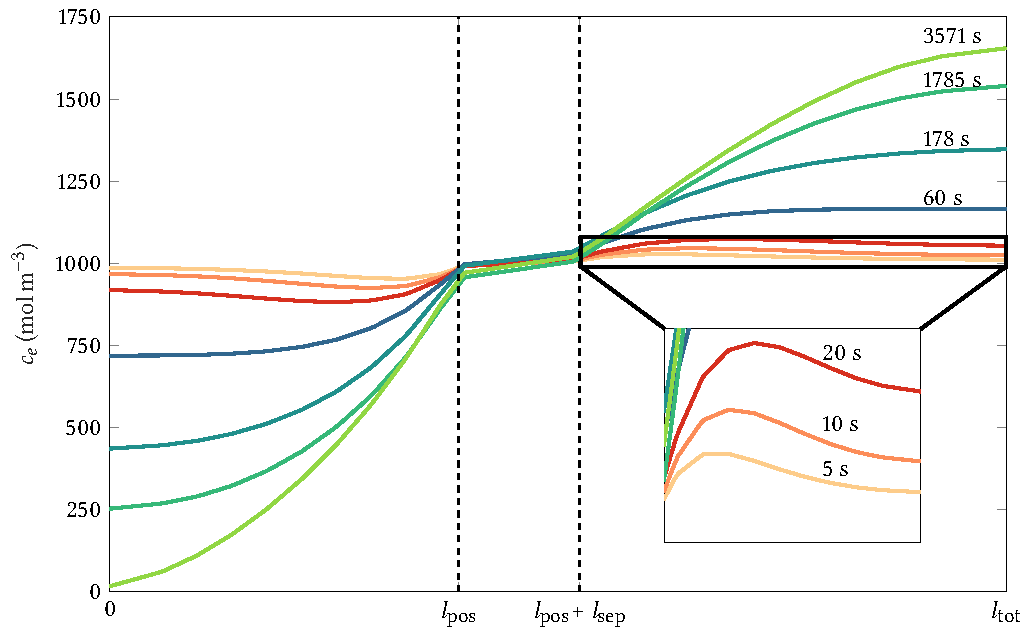
\includegraphics{ce_1C_at_various_times.pdf}
    \caption[Electrolyte conc.\ (time-snapshots) along cell thickness for 1C~discharge]{\ch{Li^+}~ion concentration in electrolyte along cell thickness
        at various time-snapshots during a 1C~discharge simulation of the
        \glsfmtshort{p2d} model. A \glsfmtlong{qss} (\glsfmtshort{qss}) spatial
        profile  with inflection point at each separator interface begins to
        form at \approx \SI{60}{\second} after discharge begins. However, the
        ionic concentration in electrolyte exhibits a significantly different
        transient behaviour (zoomed inset) possessing another inflection point
        that disrupts the monotonic trend. Depletion of ionic concentration at
        positive current collector  towards end of discharge is also seen
    (bottom left).}
    \label{fig:ce1cdischgwithzoom}
\end{figure}

Although  not presented  in the  context  of incorporating  into the  \gls{spm},
Guduru~\etal~\cite{Guduru2012}   derived   an   analytical   solution   of   the
spatio-temporal  evolution  of  electrolyte concentration  using  the  \gls{sov}
method.  The \gls{sov}  method was  first applied  to modelling  of lithium  ion
cells  by Subramanian~\etal~\cite{Subramanian2001a}  to  solve  for solid  phase
concentration  profiles in  spherical  electrode particles.  Although the  ionic
concentration  in  the electrolyte  computed  by  the analytical  expression  in
Guduru~\etal~\cite{Guduru2012} seems like a feasible choice for inclusion into
the \gls{spm}, it is only  applicable for galvanostatic  boundary conditions
\ie~when  the applied current  is held  constant over  time. By  natural
extension,  researchers could hypothesise  that this  restriction  may  be
removed  by  considering the  input current as  piecewise constant  over small
sample  intervals. Such  a hypothesis could  be  reinforced  by  the  fact that 
standard  drivecycles  are  specified as  discrete  samples and  the 
discrete-time  \gls{spm} processes  these  input samples assuming \gls{zoh}
behaviour. However, the analytical solution presented by  Guduru and co-workers
assumes a  \gls{qss}  concentration  profile. These  authors consider  a
near-instantaneous  establishment of  this \gls{qss}  and suggest  a
parameter-independent analysis  through use of dimensionless  concentrations and
time-constants instead of absolute time.

In  the  studies  conducted  by  this  thesis  author,  significantly  different
transient  behaviour  is exhibited  by  the  electrolyte concentration  profile.
In  particular,  the time  taken  to  establish  the  \gls{qss} profile  is  not
negligible. This  difference in behaviour  could be attributed to  the different
parameter  set used.  \Cref{fig:ce1cdischgwithzoom}  shows  the spatial  profile
of  ionic  concentration at  various  snapshots  of  time during  a  1C~constant
current  discharge.  Starting  at \SI{100}{\percent}  \gls{soc},  the  discharge
lasts~\SI{3571}{\second}.  It  is seen  that  it  takes nearly  \SI{60}{\second}
to  establish  the approximately  parabolic  shape  assumed by  the  electrolyte
concentration. After the initial transient has elapsed, the underlying structure
of the mathematical equations can be assumed  to be static. This is evidenced by
the  fact  that  at  \SI{1785}{\second}  \ie~after  half  of  the  discharge  is
completed, the shape of the curve is  nearly identical to the one towards end of
discharge. These  \gls{qss} curves  have their sole  inflection points  at their
separator  interfaces and  remains monotonic  within their  respective electrode
regions.  The  difference in  height  for  various  times  can be  accounted  by
the  coefficients  solved  using  the  analytical  modal  solution  proposed  in
Guduru~\etal{}.

The  axes  in  the  inset of  \cref{fig:ce1cdischgwithzoom}  shows  a  zoomed-in
view  of  the electrolyte  concentration  during  the transient  phase,  wherein
the  \gls{qss}  has  not  yet  been  established.  In  particular,  there  exist
additional inflection points,  one within the interior of  each electrode, which
render the transient concentration  profile mathematically incompatible with the
monotonicity  exhibited  by  the  \gls{qss} profile.  Thus,  in  highly  dynamic
operating  conditions with  frequent reversals  in  the direct  of current,  the
\gls{qss} assumption for the galvanostatic analytical solution becomes harder to
uphold without introducing significant  errors. Finally, the analytical solution
profile in Guduru~\etal{}  is not amenable to embedded  implementation, since it
consists of a set of non-trivial trigonometric computations at each time-step.

Prada~\etal~\cite{Prada2012} were  the first to provide  a simplified expression
for potential drop in the electrolyte  by including the terms representing ionic
concentration gradient within the cell thickness. Thus, \cref{eq:electrolytepd}
gets modified as
\begin{equation}\label{eq:electrolytepdwithce}
    \phi_\epos - \phi_\eneg = (1-t_{+}^0) \frac{2RT}{F}\ln \frac{c_\text{e,\tiny pos/cc}}{c_\text{e,\tiny neg/cc}}-\frac{I}{2 A}\left(\frac{l_\text{neg}}{\kappa_\text{eff,neg}} + 2 \frac{l_\text{sep}}{\kappa_\text{eff,sep}} + \frac{l_\text{pos}}{\kappa_\text{eff,pos}}\right)
\end{equation}
Although the complete expression for  electrolyte overpotential was provided, it
was  presented in  a cursory  manner \ie~without  detailing the  spatio-temporal
computation   of   ionic  concentration   values   at   the  current   collector
interfaces.  Nevertheless,  it  is  important   to  note  this  contribution  as
\cref{eq:electrolytepdwithce} is widely relied upon by subsequent literature and
shall be used in \cref{subsec:electrolyteopcalc}.

% in the original work of electrolyte concentration distributio presented by thisn
% thesis author i                                                                n


The  pioneering  work by  Rahimian~\etal{}~\cite{KhaleghiRahimian2013}  provided
approximate  expressions for  \emph{both}  charge transport  and mass  transport
properties of the electrolyte specifically with the focus on improving the basic
\gls{spm}. These  authors discuss  the usage of  a polynomial  approximation for
electrolyte concentration and potentials. In  particular, a cubic polynomial was
chosen  for  approximating  the  electrolyte  concentration  within  the  porous
electrodes.  This  necessitates  the  need   to  solve  for  eight  coefficients
for  uniquely  describing  the  electrolyte  concentration  profile  within  the
electrode  regions. However,  in the  standard  \gls{dfn} model,  the number  of
electrolyte-specific  \glspl{pde} and  their  corresponding boundary  conditions
describing charge and  mass transport is insufficient to uniquely  solve for all
unknown coefficients of this polynomial approximation. A detailed explanation of
this equation deficiency shall be discussed in \cref{subsec:symbolicreg}.


To overcome the issue of  equation deficiency, Rahimian~\etal{} adopted a scheme
wherein one  additional spatial location in  the interior of each  electrode was
also needed. The coefficients of the polynomial approximation were then obtained
by iteratively solving a large  coupled system of algebraic equations, embedding
within  them  the additional  equations  evaluated  at  the interior  points.  A
complicating issue  that arises  is regarding the  optimal positioning  of these
additional interior  points. An online  numerical optimisation was  performed to
obtain  the optimal  placement of  this interior  node. In  the opinion  of this
thesis author, these optimisation results could be sensitive to the thickness of
the electrodes  among other  parameters. A  discussion of  the stability  of the
proposed  routine and  its  robustness  to parameter  variations  shall help  in
lending confidence in  the proposed method. Although sufficient  accuracy of the
improved \gls{spm} was demonstrated for currents up to 5C, a notable omission is
the  discussion  of  the  model's  performance to  dynamic  input  profiles.  In
conclusion, the author  of this thesis opines that, although  this method serves
as  a  proof  of  concept towards  implementing  polynomial  approximations  for
electrolyte dynamics, until the aforementioned  gaps are addressed with clarity,
it is not convincing for uptake by relevant stakeholders.

Kemper  and  Kum~\cite{Kemper2013} presented  an  approach  wherein the  spatial
gradients  of the  electrolyte concentration  are neglected.  The time-evolution
of  \emph{average}  ionic  concentration  in  each of  the  three  cell  regions
\viz~positive electrode,  separator and  negative electrode  are described  by a
set  of three  \glspl{ode}.  As  established by  the  discussion  thus far,  the
concentration gradients  along the axial  thickness of the cell  is significant,
even at  moderate {C-rates}.  Lending strength  to doubts  on the  model's wider
applicability  is the  fact that  results  from constant  current inputs  (which
induce large concentration  gradients in electrolyte) have not  been reported in
this work. Thus,  this approach is deemed as not  satisfactory enough to warrant
further engagement.

Luo~\etal~\cite{Luo2013} derived  a parabolic  approximation of  the electrolyte
concentration  distribution along  the  thickness of  the  cell. The  derivation
is  obtained  for  the case  of  steady-state  wherein  the  rate of  change  of
concentration  is  zero.  However,  the  author  of  this  thesis  is  sceptical
about  this  since  in  the  set of  independent  simulations  conducted,  there
was  no  situation  other  than  prior  to  application  of  current  that  this
exact  steady-state condition  is satisfied.  In the  \gls{qss} profile  concept
discussion based  on \cref{fig:ce1cdischgwithzoom},  it is  clear that  only the
\emph{spatial} profile  reaches a shape that  can be potentially described  by a
mathematically  invariant family  of  curves. The  electrolyte concentration  is
still  \emph{time-varying}  and  therefore violates  the  static  time-evolution
assumption.  Although  Luo~\etal~\cite{Luo2013}  do not  explicitly  acknowledge
this,  they  do  provide  an  extension  for  general  operating  conditions  by
introducing  two  exponential   scaling  functions~$f_n(t)$  and~$f_p(t)$  while
retaining  the assumption  of parabolic  spatial behaviour.  The computation  of
certain time-constants in these scaling functions are not elucidated nor are the
procedural  steps  for determination  of  the  aforementioned scaling  functions
provided.


In a  subsequent paper  by the  same authors  \ie~Luo~\etal~\cite{Luo2013a}, the
electrolyte concentration  model together  with a  similarly-derived electrolyte
potential model  was incorporated into  the conventional \gls{spm} to  arrive at
what the  authors term  as extended~\gls{spm}. In  the aforementioned  work, the
electrolyte potential is set to account for contribution from two terms ---
\begin{enumerate*}[label=\emph{\alph*})]
    \item ohmic drop due to bulk solution resistance, and
    \item polarisation potential due to concentration gradients
\end{enumerate*}
Although it  seeks to correctly account  for the two causes  of overpotential in
the  electrolyte,  there  is  no  detailed explanation  on  the  computation  of
quantities such as time-constants involved in the polarisation potential term.

A modified version of the electrolyte model proposed in Luo~\etal~\cite{Luo2013}
was  used  in Zou~\etal~\cite{Zou2016a}  for  observer  design in  an  \gls{soc}
estimation application. The modification  essentially consists of truncating the
complex expression  in Luo~\etal~\cite{Luo2013},  which originally  consisted of
six  coefficients  $p_1$~through~$p_6$  to  just two,  and  elimination  of  the
aforementioned time-constants. However,  to the disappointment of  the author of
this thesis, the claim that truncation  to~$n=2$ terms is sufficient to describe
the dynamics  proved to be  optimistic for the  parameter set considered.  In my
attempts  to reproduce  this work,  an arbitrary  scaling factor  was needed  to
correct for the electrolyte potential  drop and match the \gls{p2d} simulations.
The requirement for such scaling factors  whose physical origins are not clearly
identifiable lends to scepticism on  the model's robustness. Furthermore, it was
found that  this value  needed to  be hand-tuned  for each  parameter-set. Until
these gaps are addressed clearly, it  is worth seeking other viable alternatives
to model the electrolyte dynamics of the cell.

After  completing  the  simulations  with  the  aforementioned  scaling  factors
and  continuing  in  the  quest  for other  alternatives,  the  author  of  this
thesis  made  an observation  that  other  researchers  have  had to  resort  to
similar techniques  for describing the electrolyte  overpotential. For instance,
Han~\etal~\cite{Han2015a} use  a similar  scaling factor~${p<0}$ for  the entire
expression   of  \cref{eq:electrolytepdwithce}   representing  the   electrolyte
overpotential   using  the   polynomial  approximation   approach  proposed   by
Rahimian~\etal~\cite{KhaleghiRahimian2013}.  However, these  unexplained scaling
factors lower the confidence regarding the model's general applicability.


Tanim~\etal~\cite{Tanim2014}  accounted  for  electrolyte dynamics  by  deriving
reduced  order  transfer  functions  for ionic  concentration  distribution  and
electrolyte   overpotential  using   the  \gls{ima}   technique.  However,   the
coefficients  of these  transfer functions  are excessively  long and  comprised
of  chained algebraic  operations  expressed in  a high-entropy  sum-of-products
form   in  the   appendix  of   the   aforesaid  article.   For  instance,   ten
coefficients  are  needed  to  describe  the  concentration  profile  while  six
coefficients  are required  for  the electrolyte  potential.  The median  length
of  each  atomic  sub-expression  of these  coefficients  is  sufficiently  high
to  obfuscate   their  physical  significance.   A  low-entropy  form   for  the
coefficients  of  these   transfer  functions  similar  to   that  pioneered  by
Middlebrook~\cite{Middlebrook} and  exemplified in the  design-oriented analysis
of  electric   circuits~\cite{Middlebrook1998,Vorperian2002}  could   have  been
helpful to aid the readers' understanding.  The author of this thesis recognises
that  mathematical complexity  should  not be  the sole  basis  to evaluate  the
merits of  such proposed improvements.  Although the presentation of  these long
coefficients  have been  judiciously moved  to the  appendix, their  derivations
---  essential to  prove  the model's  validity ---  is  curiously omitted.  The
unwieldiness  of the  mathematical expressions  presented therein  increases the
probabilities of introducing human errors during implementation.

It  is worth  noting that  Marcicki~\etal~\cite{Marcicki2013} had  independently
proposed  a similar  approach \viz~deriving  a transcendental  transfer function
from  electrolyte  concentration  to  applied  current, albeit  for  a  cell  of
\gls{lfp} chemistry. This transfer function  consisted of a series of hyperbolic
trigonometric functions which  were later truncated by  Padé approximation (see
\cref{subsec:freqdomainroms}  for  a  brief  introduction  to  frequency  domain
\glspl{rom}).  However,  upon the  trial  of  this  approach for  the  \gls{lco}
parameter  set (see  \cref{tbl:lcoSimParamsSPMp2d}) by  this thesis'  author, in
order to obtain sufficient accuracy, the truncation order had to be raised to at
least seven, similar in complexity  to that of Tanim~\etal~\cite{Tanim2014a}. In
both  Marcicki~\etal~\cite{Marcicki2013} and  Tanim~\etal~\cite{Tanim2014a}, the
electrolyte-specific enhancements to the \gls{spm}  are in the frequency domain,
placing  further burden,  particularly  on industry  stakeholders to  accurately
interpret and  transform the  coefficients to  a time-domain  implementation for
deployment  in an  embedded  \gls{bms}.  Owing to  this,  as  already stated  in
\cref{subsec:freqdomainroms},  these  models  fall  outside the  scope  of  this
thesis.

% ignoring prof plett's latest work on electrolyte transfer functions

Fan~\etal~\cite{Fan2016}   proposed   an   Extended  \gls{spm}   that   includes
electrolyte dynamics using  the \gls{gpm} which achieves  an acceptable accuracy
in terminal voltage performance. Although these authors claim that the \gls{gpm}
is computationally  \emph{cheaper} than  other model order  reduction techniques
such as proper orthogonal decomposition  and balanced truncation, this claim has
not been substantiated. The sole comparison of \gls{cpu} times presented in this
work  only compares  the  \gls{gpm} against  the  classical \gls{fdm}.  Although
an  impressive  computational speed  is  achieved,  it  is unclear  whether  the
model equations,  particularly those involving solutions  of non-linear integral
expressions  resulting from  applying the  Galerkin's  method can  be solved  in
real-time for  embedded implementation.  It appears that  the \gls{gpm}  is more
suitable for desktop simulations. In  congruence with my scepticism, the authors
of Fan~\etal~\cite{Fan2016} have  not claimed the suitability of  their work for
online/embedded  application  in a  \gls{bms}.  Therefore,  as per  this  thesis
authors' stance  explained in \cref{sec:classificationscheme},  models employing
such methods are deemed to be not in alignment with the goals of this thesis.

Moura~\etal~\cite{Moura2017} proposed an improved \gls{spm} by simply augmenting
the  conventional  \gls{spm}  with  a simplified  form  of  electrolyte-specific
equations of  the original  \gls{dfn} model. The  resulting model  therefore has
\glspl{pde} in it and therefore not easily amenable for embedded implementation.
Lotfi~\etal~\cite{Lotfi2017}  presented  an   algebraic  approximation  for  the
spatial  distribution   of  electrolyte  concentration  by   modifying  standard
parabolic expressions with leading exponential  coefficients. There are two main
issues with this approach. It is  not explained why that particular mathematical
formulation was chosen. For instance, its superiority over other feasible family
of  curves is  not discussed.  Secondly, the  aforesaid coefficients  are to  be
determined through  solution of  equations obtained  by applying  continuity and
flux boundary conditions from the \gls{dfn} model for electrolyte concentrations
at  the  electrode-separator   interfaces.  Since  exponential-type  expressions
are  assumed  in the  aforesaid  mathematical  formulations, the  resulting  set
of  equations  are  non-linear,  the  solving  of which  in  the  context  of  a
resource-constrained environment is problematic.

\Cref{tbl:spmlassificationlittreviewsummary} provides a summary of the  salient
electrolyte enhanced \glspl{spm} from literature.

 % -*- root: ../../main.tex -*-
%!TEX root = ../../main.tex

% \setlength\LTleft{0pt}
% \setlength\LTright{1cm}

{% begin box to localize effect of arraystretch change
% \setlength\tymin{.25\textwidth}
\setlength{\LTpre}{-5pt}
\singlespacing
\renewcommand{\arraystretch}{1.50}
\small
\centering
\begin{ltabulary}[c]{@{} l L L @{}}
    \caption
    {%
    Summary of salient literature on electrolyte enhanced \glsfmtshortpl{spm} 
    }\label{tbl:spmlassificationlittreviewsummary}\\
    \toprule
    \multicolumn{1}{c}{Source} & \multicolumn{1}{c}{Key Contributions} & \makecell{Limitations/ \\ Other Remarks} \\        
    \midrule
    \endfirsthead
    \multicolumn{3}{c}%
    {{\normalsize \bfseries \tablename\ \thetable{} --- \normalfont  continued from previous page}} \\
    \toprule
    \multicolumn{1}{c}{Source} & \multicolumn{1}{c}{Key Contributions} & \makecell{Limitations/ \\ Other Remarks} \\
    \midrule
    \endhead
    \midrule
    \multicolumn{3}{ r @{}}{{\normalsize  Continued on next page}} \\[-0.5ex]
    \bottomrule
    \endfoot

    \bottomrule
    \endlastfoot

    Schmidt~\etal~\cite{Schmidt2010c} & {Electrolyte concentration solved by an eigenfunction expansion for spatial profile and an \gls{ode} solution for temporal dynamics} & {Excessive theoretical emphasis without regular contextual references to cell modelling, which hinders reproducibility} \\
    Guo~\etal~\cite{Guo2011a} & {Non-linear resistance as a function of current and temperature to capture electrolyte overpotential} & {Empirical approach which is difficult to generalise across parameter sets since large corrections of the order of a few \si{\milli\volt} become essential; Non-linear optimisation may converge to a local minimum} \\
    Di~Domenico~\etal~\cite{DiDomenico2010} & {First to present an approximate analytical solution for electrolyte overpotential} & {Lacks discussion on spatio-temporal calculation of ionic concentration; presumably used constant initial value which is problematic with sustained unidirectional currents} \\
    Guduru~\etal~\cite{DiDomenico2010} & {Pioneered an analytical solution for the spatio-temporal evolution of electrolyte concentration using the \glsfirst{sov} method} & {The derived analytical solution is applicable only for galvanostatic discharge; assumption of near instantaneous establishment of \gls{qss} hinders extensions using \gls{pwl} approximations while trigonometric computations at each time-step impacts embedded applicability} \\
    Prada~\etal~\cite{Prada2012} & {First to incorporate polarisation due to ionic diffusion in the expression for electrolyte overpotential} & {The solution of spatio-temporal ionic concentration is not detailed. However, post-computation of this term, the equation in Prada~\etal~\cite{Prada2012} is widely used for the electrolyte overpotential contribution to cell terminal voltage} \\
    Rahimian~\etal~\cite{KhaleghiRahimian2013} & {Cubic polynomials for spatial approximation of electrolyte concentration and demonstrated satisfactory accuracy for currents up to 5C} & {Limited by the issue of equation deficiency in the \gls{p2d} model; proposed workaround involves computations at additional interior points which is determined by an expensive placement optimisation algorithm} \\
    Luo~\etal~\cite{Luo2013,Luo2013a} & {Derived a modified parabolic  approximation (with exponential scaling functions) for electrolyte spatial concentration profile} & {Computation of time constants of the exponential scaling functions is not explained; improvements over a standard quadratic approximation model is not elucidated} \\
    Tanim~\etal~\cite{Tanim2014} & {Derived transfer functions for ionic concentration distribution and electrolyte overpotential using \glsfmtlong{ima}} & {Coefficients of transfer functions are excessively long and mathematically intractable; Is based upon many high entropy expressions whose analytical derivations are omitted} \\
\end{ltabulary}
}% end box



% The other main contribution of this work is its feasibility analysis of having
% convergent  estimators for  this model  and design  of such  a \gls{pde}-based
% estimator.  In  the  views of  this  thesis  author,  this  approach is  on  a
% trajectory that deviates  too far from a simplified model  suitable for online
% implementation.


% Therefore, my analysis  on the quadratic approximation  method for electrolyte
% concentration is presented next in \cref{sec:quadraticapprox}.


% May also mention some typographical errors  in Lotfi etal second paper Mention
% that parabolic profile is a common theme  perhaps it cannot be done, but we do
% not give up. Equation deficiency

% But  I did  something different.  The high  accuracy of  the \gls{soc}  in the
% basic  \gls{spm} leads  to the  author's  hypothesis that  if the  electrolyte
% concentration  can be  solved  as an  independent  subsystem and  incorporated
% into  the terminal  voltage,  this  can lead  to  an  improved \gls{spm}  with
% electrolyte dynamics.  Such a decoupled  electrolyte inclusion into  the basic
% \gls{spm}\fxnote{fix this sentence}



\subsection{Conclusions}

A survey  of the  recent  literature dealing with  the \gls{spm}  family of
models reveals a diminishing rate of advancement in quantifiable improvements to
the underlying plant model itself. This nearly-static trend can be attributed to
the general  consensus within the  research community  that these models  may be
too  simplistic  and  not  of  suitable accuracy  to  warrant  further  studies.
Other  than a  small  minority  of papers  that  either  propose core  modelling
improvements  to tackle  their inaccuracies,  or add new  enhancements such  as
mechanical-stress  physics~\cite{Li2017a,Li2018b}, latest  work  in this  family
of  models predominantly  pertains  to  their application  in  areas like  state
estimation~\cite{Chaochun2018,Lin2017,Tran2017,Moura2017,Zou2016a},      optimal
charging~\cite{Perez2017,Perez2017a},    cycling    performance~\cite{Maia2017},
conversion           to            equivalent           circuits~\cite{Li2017b},
parametrisation~\cite{Li2018,Rajabloo2017,Bizeray2017,Namor2017}, pack-balancing
studies~\cite{Docimo2018a}  and   observer  design  for   joint  state-parameter
estimation~\cite{Ascencio2016}. The \gls{spm} approach  has also been extended
to the case of  composite electrodes, leading to  a state estimator design 
after basic observability  analysis~\cite{Bartlett2015}.   Owing  to  their 
simplicity,  this thesis author believes that \glspl{spm} hold the highest
potential to bring physics-based models to embedded \glspl{bms}. With this goal 
in view, this thesis seeks to resurrect interest in \glspl{spm} by addressing the
recent paucity in fundamental modelling improvements. 

% However, prior to doing  this, a complete analysis
% identifying the strengths and  weaknesses of the salient  models within the
% \gls{spm}  family is warranted which is performed in \cref{ch:spmanalysis}.

Based upon the thesis author's experiences in  trying to  replicate the  results
from the  literature presented in \cref{sec:electrolyteinclusion}, any
questionable elements in such prior efforts can be  attributed to  inaccuracies
in  estimating the  spatio-temporal evolution of  electrolyte   concentration. 
Upon   obtaining  a  good  estimate   of  the electrolyte concentration profile,
\cref{eq:electrolytepdwithce} is deemed to be satisfactory  for the  electrolyte
overpotential  computation. Thus,  it can  be concluded that the focus of
research efforts must be  on accurate determination of the electrolyte
concentration profile.

Analysing the literature presented in \cref{sec:electrolyteinclusion}, it can be
seen that the proposed enhancements to computing the  ionic concentration 
in electrolyte  falls into  one of  the following two categories
\begin{itemize}[topsep=0pt,partopsep=0pt,itemsep=0pt]
    \item model description through physical principles followed by mathematical
        simplification
    \item fitting of pre-assumed simplified mathematical structures to some
        physical phenomena
\end{itemize}

In   the  author's   view,   it   appears  that   using   the  former   approach
yields  technically  correct,  yet  mathematically  convoluted  expressions  for
overpotentials that  are fraught with implementation  difficulties. Although the
latter  approach looks  promising  in  terms of  ease  of implementation,  their
sub-optimal  performance  and lack  of  wider-applicability  leaves much  to  be
desired.  Among  the latter  class  of  models,  owing  to its  simplicity,  the
quadratic (parabolic)  approximation method for electrolyte  concentration is an
attractive option. It is therefore important  to perform an in-depth analysis of
this sub-class  of models and  understand their source of  potential weaknesses.
Such  an analysis  has  yet  not been  performed  in  literature and is
therefore presented in \cref{sec:quadraticapprox}.


This concludes  the author's review of  literature of the various  reduced order
modelling  strategies. Based  on the  wealth  of information  gleaned from  this
study,  it was  possible to  make  an informed  choice to  pursue the  \gls{spm}
approach  for further  research.  In particular,  it came  to  light that  there
has  been  no systematic  analysis  of  the  state  of the  art  \gls{spm}-based
approach with  a view  to quantify their  performance boundaries.  This author's
contributions to  the time-domain  implementation-focus reduced  order modelling
field include
\begin{itemize}[noitemsep,topsep=0pt, before={\vspace*{-0.25\baselineskip}}]
    \item a thorough analysis of the existing \gls{spm} variants ranging from the rudimentary to the sophisticated
    \item enumeration of issues plaguing each \gls{spm} variant, including current state of the art
    \item further evaluation of literature on the current tactics to overcome the current challenges along with their associated drawbacks
    \item conducting a  wide range of hypotheses-driven trials in an attempt to enhance  the basic \gls{spm} (some of which did not yield the desired
        improvements), and
    \item arriving at  a  feasible  approach  capable  of  moulding  the
        \gls{spm}  framework into  a  readily implementable  solution in
        electric vehicle applications
\end{itemize}
This research was  performed through an iterative cycle of  analysis, design and
simulation-based verification  and shall be  elucidated in a  discourse spanning
two chapters \viz~\cref{ch:spmanalysis} and \cref{ch:newelectrolytemodel}.

